\documentclass{beamer}
\usepackage{tikz}
\usepackage[english]{babel}
\usepackage{proof}
\usetheme{Luebeck}
\usetikzlibrary{positioning}
\usetikzlibrary{decorations.pathreplacing}
\definecolor{darkblue}{rgb}{0,0,.803}
\definecolor{cream}{rgb}{1,1,.8}

\newcommand{\smath}[1]{\textcolor{darkblue}{\ensuremath{#1}}}
\newcommand{\dn}{\stackrel{\mbox{\scriptsize def}}{=}}
\newcommand{\Zero}{{\bf 0}}
\newcommand{\One}{{\bf 1}}

\newenvironment{bubble}[1][]{%
\addtolength{\leftmargini}{4mm}%
\begin{tikzpicture}[baseline=(current bounding box.north)]%
\draw (0,0) node[inner sep=2mm,fill=cream,ultra thick,draw=red,rounded corners=2mm]% 
\bgroup\begin{minipage}{#1}\raggedright{}}
{\end{minipage}\egroup;%
\end{tikzpicture}\bigskip}

\newcommand\grid[1]{%
	\begin{tikzpicture}[baseline=(char.base)]
	\path[use as bounding box]
	(0,0) rectangle (1em,1em);
	\draw[red!50, fill=red!20]
	(0,0) rectangle (1em,1em);
	\node[inner sep=1pt,anchor=base west]
	(char) at (0em,\gridraiseamount) {#1};
	\end{tikzpicture}}
\newcommand\gridraiseamount{0.12em}

\makeatletter
\newcommand\Grid[1]{%
	\@tfor\z:=#1\do{\grid{\z}}}
\makeatother	

\newcommand\Vspace[1][.3em]{%
	\mbox{\kern.06em\vrule height.3ex}%
	\vbox{\hrule width#1}%
	\hbox{\vrule height.3ex}}

\def\VS{\Vspace[0.6em]}


\title[POSIX Lexing with Derivatives of Regexes]
{\bf POSIX Lexing with\\ 
	\bf Derivatives of Regular Expressions\\
	\bf (Proof Pearl)}
\author{Fahad Ausaf, Roy Dyckhoff and Christian Urban}
\date{King's College London, University of St Andrews}


\begin{document}
\maketitle


    %%%%%%%%%%%%%%%%%%%%%%%%%%%%%%%%%%%%%%%%%%%%%%%%%%%%%%%%%%%%%
	\begin{frame}
	\frametitle{Brzozowski's Derivatives of Regular Expressions}
		
	Idea: If \smath{r} matches the string \smath{c\!::\!s}, 
	what is a regular expression that matches just \smath{s}? \\
		
   \begin{center}
   \begin{tabular}{l@{\hspace{5mm}}lcl}	
   chars:
   &\smath{\Zero \backslash c} & \smath{\dn} & \smath{\Zero}\\
   &\smath{\One \backslash c}  & \smath{\dn} & \smath{\Zero}\\
   &\smath{d \backslash c}  & \smath{\dn} & 
   \smath{\textit{if}\;d = c\;\textit{then}\;\One\;\textit{else}\;\Zero}\\
   &\smath{r_1 + r_2 \backslash c} & \smath{\dn} & 
   \smath{r_1 \backslash c \,+\, r_2 \backslash c}\\
   &\smath{r_1 \cdot r_2 \backslash c} & \smath{\dn} & 
   \smath{\textit{if}\;\textit{nullable}\;r_1}\\
   && & \smath{\textit{then}\;r_1\backslash c \cdot r_2 \,+\, r_2\backslash c
   \;\textit{else}\;r_1\backslash c \cdot r_2}\\
   &\smath{r^* \backslash c} & \smath{\dn} & 
   \smath{r\backslash c \,\cdot\, r^*}\bigskip\\
   
   strings:
   &\smath{r\backslash []} & \smath{\dn} & \smath{r}\\  
   &\smath{r\backslash c\!::\!s} & \smath{\dn} & 
   \smath{(r\backslash c)\backslash s}\\
   \end{tabular}
   \end{center}
	\end{frame}
	
	%%%%%%%%%%%%%%%%%%%%%%%%%%%%%%%%%%%%%%%%%%%%%%%%%%%%%%%%%%%%%
	
	\begin{frame}
	\frametitle{Brzozowski's Matcher}
	
	Does \smath{r_1} match string \smath{abc}? 
	
	\begin{center}
	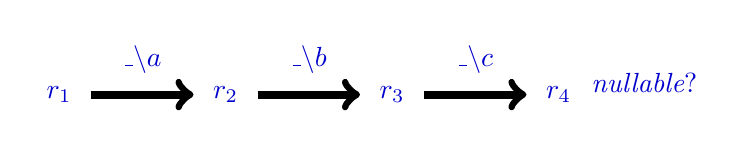
\begin{tikzpicture}[scale=2,node distance=1.3cm,every node/.style={minimum size=8mm}]
		\node (r1)  {\smath{r_1}};
		\node (r2) [right=of r1] {\smath{r_2}};
		\draw[->,line width=1mm]  (r1) -- (r2) node[above,midway] {\smath{\_\backslash a}};
		\node (r3) [right=of r2] {\smath{r_3}};
		\draw[->,line width=1mm]  (r2) -- (r3) node[above,midway] {\smath{\_\backslash b}};
		\node (r4) [right=of r3] {\smath{r_4}};
		\draw[->,line width=1mm]  (r3) -- (r4) node[above,midway] {\smath{\_\backslash c}};
		\draw (r4) node[anchor=west] {\;\raisebox{3mm}{\smath{\;\;\textit{nullable}?}}};
	\end{tikzpicture}
	\end{center}\pause
	
	It leads to an elegant functional program:
	
	\begin{center}
	\smath{\textit{matches}\,(r, s) \dn \textit{nullable}\,(r\backslash s)}
	\end{center}\pause
	
	It is an easy exercise to formally prove (e.g.~Coq, HOL, Isabelle):
		
	\begin{center}	
		\smath{\textit{matches}\,(r, s)} if and only if 
		\smath{s \in L(r)}
   \end{center}\pause 
		
	{\bf But Brzozowski's matcher gives only a yes/no-answer.}	
	\end{frame}
	
	%%%%%%%%%%%%%%%%%%%%%%%%%%%%%%%%%%%%%%%%%%%%%%%%%%%%%%%%%%%%%
	
%	\begin{frame}
%		\frametitle{Sulzmann and Lu's Matcher}
%		\begin{itemize}
%			\item Sulzmann \& Lu came up with a beautiful idea for how 
%			to extend the simple regular expression matcher to POSIX 
%			matching/lexing (FLOPS 2014)
%			\item The idea: define an inverse operation to the derivatives
%		\end{itemize}
%	\end{frame}
	
	%%%%%%%%%%%%%%%%%%%%%%%%%%%%%%%%%%%%%%%%%%%%%%%%%%%%%%%%%%%%%%
	
	\begin{frame}
	\frametitle{Sulzmann and Lu's Matcher}

   Sulzmann and Lu added a second phase in order to answer
   \alert{\textbf{how}} the regular expression matched the string.
   
   \begin{center}\small
   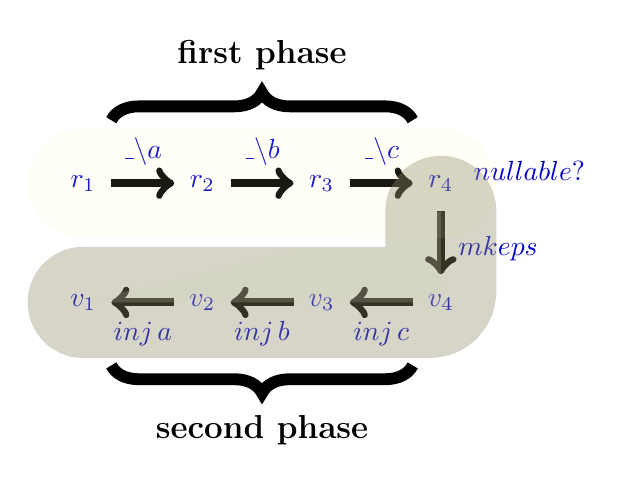
\begin{tikzpicture}[scale=1,node distance=0.8cm,every node/.style={minimum size=7mm}]
		\node (r1)  {\smath{r_1}};
		\node (r2) [right=of r1] {\smath{r_2}};
		\draw[->,line width=1mm]  (r1) -- (r2) node[above,midway] {\smath{\_\backslash a}};
		\node (r3) [right=of r2] {\smath{r_3}};
		\draw[->,line width=1mm]  (r2) -- (r3) node[above,midway] {\smath{\_\backslash b}};
		\node (r4) [right=of r3] {\smath{r_4}};
		\draw[->,line width=1mm]  (r3) -- (r4) node[above,midway] {\smath{\_\backslash c}};
		\draw (r4) node[anchor=west] {\;\raisebox{3mm}{\smath{\;\;nullable?}}};
		\node (v4) [below=of r4] {\smath{v_4}};
		\draw[->,line width=1mm]  (r4) -- (v4);
		\node (v3) [left=of v4] {\smath{v_3}};
		\draw[->,line width=1mm]  (v4) -- (v3) node[below,midway] {\smath{inj\,c}};
		\node (v2) [left=of v3] {\smath{v_2}};
		\draw[->,line width=1mm]  (v3) -- (v2) node[below,midway] {\smath{inj\,b}};
		\node (v1) [left=of v2] {\smath{v_1}};
		\draw[->,line width=1mm]  (v2) -- (v1) node[below,midway] {\smath{inj\,a}};
		\draw (r4) node[anchor=north west] {\;\raisebox{-8mm}{\smath{mkeps}}};

       \draw [decorate,decoration={brace,amplitude=10pt,raise=8mm},
              line width=1.5mm]
              (r1) -- (r4) node [black,midway,above, yshift=12mm] 
             {\large\bf  first phase};
       \draw [decorate,decoration={brace,amplitude=10pt,raise=8mm},
              line width=1.5mm]
              (v4) -- (v1) node [black,midway,below, yshift=-12mm] 
             {\large\bf  second phase}; 
       %% first phase      
       \draw[line width=14mm, rounded corners, opacity=0.1,
             cap=round,join=round,color=yellow!30]
            (r1.center)  -- (r4.center);
       %% second phase     
       \draw[line width=14.1mm, rounded corners, opacity=0.2,
             cap=round,join=round,draw=black, fill=white]
            (r4)  -- (v4.center) -- (v1.center);
       \draw[line width=14mm, rounded corners, opacity=0.2,
             cap=round,join=round,color=yellow!30]
            (r4)  -- (v4.center) -- (v1.center);     
	\end{tikzpicture}
   \end{center}
   
   There are several possible answers for 
   \alert{\textbf{how}}: POSIX, GREEDY, \ldots

   \end{frame}


	%%%%%%%%%%%%%%%%%%%%%%%%%%%%%%%%%%%%%%%%%%%%%%%%%%%%%%%%%%%%%
	
	\begin{frame}
	\frametitle{POSIX Matching (needed for Lexing)}


    \begin{bubble}[10cm]
    {\bf Longest Match Rule:} The longest 
    initial substring matched by any regular expression is taken 
    as the next token.
    \end{bubble}
    
    \begin{bubble}[10cm]
    {\bf Rule Priority:} For a particular longest initial substring, 
    the first regular expression that can match determines the 
	token.
    \end{bubble}
  
	For example: \smath{r_{keywords} + r_{identifiers}}

		\begin{itemize}
			\item \smath{\texttt{\Grid{iffoo\VS bla}}} 
			
			\item \smath{\texttt{\Grid{if\VS bla}}}
		\end{itemize}	
	
	\end{frame}
	
	
	
	%%%%%%%%%%%%%%%%%%%%%%%%%%%%%%%%%%%%%%%%%%%%%%%%%%%%%%%%%%%%%
	
	\begin{frame}
	\frametitle{Problems with POSIX}
	
	Grathwohl, Henglein and Rasmussen wrote:
	
	\begin{bubble}[10cm]   
	\it ``The POSIX strategy is more complicated than the greedy because 
	of the dependence on information 
	about the length of matched strings in the various subexpressions.''   
	\end{bubble}\bigskip   
	
	Also Kuklewicz maintains a unit-test repository for POSIX
	matching, which indicates that most POSIX matchcers are buggy.
	
	\begin{center}
	\url{http://www.haskell.org/haskellwiki/Regex_Posix}
   \end{center}

	\end{frame}
	
	%%%%%%%%%%%%%%%%%%%%%%%%%%%%%%%%%%%%%%%%%%%%%%%%%%%%%%%%%%%%%
	
%	\begin{frame}
%	\frametitle{Correctness}
%	\begin{itemize}
%		\item Sulzmann \& Lu came up with a beautiful idea for how 
%		to extend the simple regular expression matcher to POSIX 
%		matching/lexing (FLOPS 2014)
%		\item The idea: define an inverse operation to the derivatives
%	\end{itemize}
%	\end{frame}

	
	
	%%%%%%%%%%%%%%%%%%%%%%%%%%%%%%%%%%%%%%%%%%%%%%%%%%%%%%%%%%%%%
	
	\begin{frame}
	\frametitle{Sulzmann and Lu Matcher}
	
	We want to match the string $abc$ using $r_1$\\
	
	\begin{center}	
		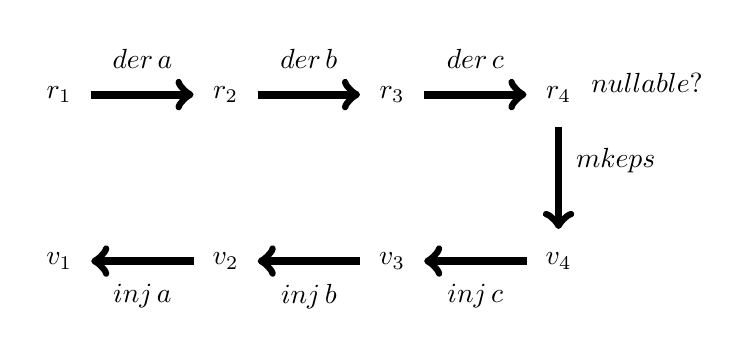
\begin{tikzpicture}[scale=2,node distance=1.3cm,every node/.style={minimum size=8mm}]
		\node (r1)  {$r_1$};
		\node (r2) [right=of r1] {$r_2$};
		\draw[->,line width=1mm]  (r1) -- (r2) node[above,midway] {$der\,a$};
		\node (r3) [right=of r2] {$r_3$};
		\draw[->,line width=1mm]  (r2) -- (r3) node[above,midway] {$der\,b$};
		\node (r4) [right=of r3] {$r_4$};
		\draw[->,line width=1mm]  (r3) -- (r4) node[above,midway] {$der\,c$};
		\draw (r4) node[anchor=west] {\;\raisebox{3mm}{$\;\;nullable?$}};\pause
		\node (v4) [below=of r4] {$v_4$};
		\draw[->,line width=1mm]  (r4) -- (v4);
		\draw (r4) node[anchor=north west] {\;\raisebox{-8mm}{$mkeps$}};\pause
		\node (v3) [left=of v4] {$v_3$};
		\draw[->,line width=1mm]  (v4) -- (v3) node[below,midway] {$inj\,c$};\pause
		\node (v2) [left=of v3] {$v_2$};
		\draw[->,line width=1mm]  (v3) -- (v2) node[below,midway] {$inj\,b$};\pause
		\node (v1) [left=of v2] {$v_1$};
		\draw[->,line width=1mm]  (v2) -- (v1) node[below,midway] {$inj\,a$};\pause
		%\draw[->,line width=0.5mm]  (r3) -- (v3);
		%\draw[->,line width=0.5mm]  (r2) -- (v2);
		%\draw[->,line width=0.5mm]  (r1) -- (v1);
		\onslide<1->
		\end{tikzpicture}
	\end{center}
	
	\end{frame}	
	
	%%%%%%%%%%%%%%%%%%%%%%%%%%%%%%%%%%%%%%%%%%%%%%%%%%%%%%%%%%%%%
	
	\begin{frame}
		\frametitle{Regular Expressions and Values}
		Regular expressions and their corresponding values (for how a 
		regular expression matched string):
		\vspace{5 mm} 
		\begin{columns}[c] % the "c" option specifies center vertical alignment
			\column{.4\textwidth} % column designated by a command
			\begin{tabular}{ l l l }
				\smath{r} & ::= 		& \smath{\Zero} 	\\
				& $\mid$	& \smath{\One} 		\\
				& $\mid$	& \smath{c} 				\\
				& $\mid$	& \smath{r_1 \cdot r_2}	\\
				& $\mid$	& \smath{r_1 + r_2}		\\ \\
				& $\mid$	& \smath{r^*}				\\
			\end{tabular}
			\column{.4\textwidth}
			\begin{tabular}{ l l l }
				
				\smath{v} & ::= 		& \\
				& $\mid$	& \smath{Empty} 			\\
				& $\mid$	& \smath{Char(c)} 		\\
				& $\mid$	& \smath{Seq(v_1\cdot v_2)}	\\
				& $\mid$	& \smath{Left(v)}		\\
				& $\mid$	& \smath{Right(v)}		\\
				& $\mid$	& \smath{[v_1,...,v_n]}
			\end{tabular}
		\end{columns}
		\vspace{5 mm}
		There is also a notion of a string behind a value $\mid v \mid$
	\end{frame}
	
	%%%%%%%%%%%%%%%%%%%%%%%%%%%%%%%%%%%%%%%%%%%%%%%%%%%%%%%%%%%%%
	
	\begin{frame}
	\frametitle{Mkeps and Injection Functions}
		
	\textbf{Mkeps Function}
	\begin{tabular}{ l l l }
		\textit{mkeps} (\textbf{1}) 		& $\dn$ & \textit{Empty} 	\\
		\textit{mkeps} ($r_1 \cdot r_2$) 	& $\dn$	& \textit{Seq} (\textit{mkeps} $r_1$) (\textit{mkeps} $r_2$)\\
		\textit{mkeps} ($r_1 + r_2$) 		& $\dn$	& \textit{if nullable $r_1$ then Left} (\textit{mkeps $r_1$})\\
											& 		& \textit{else Right} (\textit{mkeps $r_2$})\\
		\textit{mkeps} ($r^*$) 				& $\dn$	& \textit{Stars} []	\\
	\end{tabular}\\
				
	\end{frame}

	%%%%%%%%%%%%%%%%%%%%%%%%%%%%%%%%%%%%%%%%%%%%%%%%%%%%%%%%%%%%%
	
	\begin{frame}
	\frametitle{Mkeps and Injection Functions}
	
	\textbf{Injection Function}
	\begin{tabular}{ l l l }
		\textit{inj d c} () & $\dn$ & \textit{Char d}\\
		\textit{inj} ($r_1 + r_2$) \textit{c} (\textit{Left $v_1$}) & $\dn$ & \textit{Left} (\textit{inj $r_1$ c $v_1$})\\
		\textit{inj} ($r_1 + r_2$) \textit{c} (\textit{Right $v_2$}) & $\dn$ & \textit{Right} (\textit{inj $r_2$ c $v_2$})\\
		\textit{inj} ($r_1 \cdot r_2$) \textit{c} (\textit{Seq $v_1$ $v_2$}) & $\dn$ & \textit{Seq} (\textit{inj $r_1$ c $v_1$}) $v_2$\\
		\textit{inj} ($r_1 \cdot r_2$) \textit{c} (\textit{Left} (\textit{Seq $v_1$ $v_2$})) & $\dn$ & \textit{Seq} (\textit{inj $r_1$ c $v_1$}) $v_2$\\
		\textit{inj} ($r_1 \cdot r_2$) \textit{c} (\textit{Right $v_2$}) & $\dn$ & \textit{Seq} (\textit{mkeps $r_1$}) (\textit{inj $r_2$ c $v_2$})\\
		\textit{inj} ($r^*$) \textit{c} (\textit{Seq v} (\textit{Stars vs})) & $\dn$ & \textit{Stars} (\textit{inj r c v}::\textit{vs})
	\end{tabular}
	
	\end{frame}	
		
	%%%%%%%%%%%%%%%%%%%%%%%%%%%%%%%%%%%%%%%%%%%%%%%%%%%%%%%%%%%%%
	
	\begin{frame}
	\frametitle{POSIX Ordering Relation by Sulzmann \& Lu}
	
	\begin{itemize}
	\item Introduce an inductive defined ordering relation 
	$v \succ_r v'$ which captures the idea of POSIX matching.
	
	\item The algorithm returns the maximum of all possible values 
	that are possible for a regular expression.
	
	\item The idea is from a paper by Frisch \& Cardelli about 
	GREEDY matching (GREEDY = preferring instant gratification 
	to delayed repletion)
	
	%\item e.g. given $(a + (b + ab))^{*}$ and string $ab$\\
	%\begin{center}	
	%\begin{tabular}{ll}
	%GREEDY: & $[Left(a), Right(Left(b))]$\\
	%POSIX: 	& $[Right(Right(Seq(a, b)))]$
	%\end{tabular}
	%\end{center}
	
	\end{itemize}
	\end{frame}
	
	%%%%%%%%%%%%%%%%%%%%%%%%%%%%%%%%%%%%%%%%%%%%%%%%%%%%%%%%%%%%%
	
%	\begin{frame}
%	\frametitle{POSIX Ordering Relation by Sulzmann \& Lu}
%	
%	\begin{center}
%		$\infer{\vdash Empty : \epsilon}{}$\hspace{15mm}	
%		$\infer{\vdash Char(c): c}{}$\bigskip
%		
%		$\infer{\vdash Seq(v_1, v_2) : r_1\cdot r_2}{\vdash v_1 : r_1 \quad \vdash v_2 : r_2}$
%		\bigskip
%		
%		$\infer{\vdash Left(v) : r_1 + r_2}{\vdash v : r_1}$\hspace{15mm}
%		$\infer{\vdash Right(v): r_1 + r_2}{\vdash v : r_2}$\bigskip
%		
%		$\infer{\vdash [] : r^*}{}$\hspace{15mm}
%		$\infer{\vdash [v_1,\ldots, v_n] : r^*}
%		{\vdash v_1 : r \quad\ldots\quad \vdash v_n : r}$
%	\end{center}
%	
%	\end{frame}
	
	%%%%%%%%%%%%%%%%%%%%%%%%%%%%%%%%%%%%%%%%%%%%%%%%%%%%%%%%%%%%%
	
	\begin{frame}
	\frametitle{Problems}
	\begin{itemize}
	
	\item Sulzmann: \ldots Let's assume $v$ is not a $POSIX$ value, 
	then there must be another one \ldots contradiction.
	
	\item Exists ?
	\begin{center}
	$L(r) \not= \varnothing \;\Rightarrow\; \exists v.\;POSIX(v, r)$
	\end{center}
	
	\item In the sequence case 
	$Seq(v_1,v_2)\succ_{r_1\cdot r_2} Seq(v_1', v_2')$, 
	the induction hypotheses require 
	$|v_1| = |v_1'|$ and $|v_2| = |v_2'|$, but you only know 
	
	\begin{center}
	$|v_1| @ |v_2| = |v_1'| @ |v_2'|$
	\end{center}
	
	\item Although one begins with the assumption that the two 
	values have the same flattening, this cannot be maintained 
	as one descends into the induction (alternative, sequence)
		
	\end{itemize}
	\end{frame}
	
	%%%%%%%%%%%%%%%%%%%%%%%%%%%%%%%%%%%%%%%%%%%%%%%%%%%%%%%%%%%%%
	
%	\begin{frame}
%		\frametitle{Problems}
%		
%		\begin{itemize}
%			\item I have no doubt the algorithm is correct --- 
%			the problem is I do not believe their proof.
%			
%			\begin{center}
%				\small
%				``How could I miss this? Well, I was rather careless when 
%				stating this Lemma :)\smallskip
%				
%				Great example how formal machine checked proofs (and 
%				proof assistants) can help to spot flawed reasoning steps.''
%				
%			\end{center}
%			
%			\begin{center}
%				\small
%				``Well, I don't think there's any flaw. The issue is how to 
%				come up with a mechanical proof. In my world mathematical 
%				proof $=$ mechanical proof doesn't necessarily hold.''
%				
%			\end{center}
%			
%		\end{itemize}	
%		
%	\end{frame}
	
	%%%%%%%%%%%%%%%%%%%%%%%%%%%%%%%%%%%%%%%%%%%%%%%%%%%%%%%%%%%%%
	
	\begin{frame}
		\frametitle{Our Solution}
		
	\begin{itemize}
		\item A direct definition of what a POSIX value is, using the 
		relation \smath{s \in r \to v} (our specification)\bigskip
			
	\begin{center}
		\smath{\infer{[] \in \One \to Empty}{}}\hspace{15mm}
		\smath{\infer{[c] \in c \to Char(c)}{}}\bigskip\medskip
		
		\smath{\infer{s \in r_1 + r_2 \to Left(v)}
			{s \in r_1 \to v}}\hspace{10mm}
		\smath{\infer{s \in r_1 + r_2 \to Right(v)}
			{s \in r_2 \to v & s \not\in L(r_1)}}\bigskip\medskip
		
		\smath{\infer{s_1 @ s_2 \in r_1 \cdot r_2 \to Seq(v_1, v_2)}
			{\small\begin{array}{l}
					s_1 \in r_1 \to v_1 \\
					s_2 \in r_2 \to v_2 \\
					\neg(\exists s_3\,s_4.\; s_3 \not= []
					\wedge s_3 @ s_4 = s_2 \wedge
					s_1 @ s_3 \in L(r_1) \wedge
					s_4 \in L(r_2))
				\end{array}}}
				
				{\ldots}           
			\end{center}	
			
		\end{itemize}
	\end{frame}
	
	%%%%%%%%%%%%%%%%%%%%%%%%%%%%%%%%%%%%%%%%%%%%%%%%%%%%%%%%%%%%%%%%%%
	\begin{frame}[c]
	\frametitle{Properties}
	
	It is almost trival to prove:
	
	\begin{itemize}
	\item Uniqueness
	\begin{center}
	If $s \in r \to v_1$ and $s \in r \to v_2$ then
	$v_1 = v_2$
	\end{center}\bigskip
	
	\item Correctness
	\begin{center}
	$lexer(r, s) = v$ if and only if $s \in r \to v$
	\end{center}
	\end{itemize}\bigskip\bigskip\pause
	
	
	You can now start to implement optimisations and derive
	correctness proofs for them.% But we still do not know whether
%	
%	\begin{center}
%	$s \in r \to v$ 
%	\end{center}
%	
%	is a POSIX value according to Sulzmann \& Lu's definition
%	(biggest value for $s$ and $r$)
	\end{frame}
	
		%%%%%%%%%%%%%%%%%%%%%%%%%%%%%%%%%%%%%%%%%%%%%%%%%%%%%%%%%%%%%
		
		\begin{frame}
			\frametitle{Conclusions}
			
			\begin{itemize}
				
				\item Sulzmann and Lu's informal proof contained small gaps (acknowledged) but we believe it had
				also fundamental flaws\medskip
				
				\item We replaced the POSIX definition of Sulzmann \& Lu by a
				new definition (ours is inspired by work of Vansummeren,
				2006)\medskip
				
				\item Now, its a nice exercise for theorem proving\medskip
				
				\item Some optimisations need to be applied to the algorithm
				in order to become fast enough\medskip
				
				\item Can be used for lexing, is a small beautiful functional
				program
				
			\end{itemize}
		\end{frame}
		
	

\end{document}
